\documentclass[12pt, a4paper, oneside]{ctexart}
\usepackage{amsmath, amsthm, amssymb, bm, color, graphicx, geometry, mathrsfs,extarrows, braket, booktabs, array, xcolor, fontspec, appendix, float, subfigure, wrapfig, enumitem, titlesec}
\usepackage[colorlinks,linkcolor=red,anchorcolor=blue,citecolor=blue,urlcolor=blue,menucolor=black]{hyperref}

%%%% 设置中文字体 %%%%
\setCJKmainfont{方正新书宋_GBK.ttf}[BoldFont = 方正小标宋_GBK, ItalicFont = 方正楷体_GBK, BoldItalicFont = 方正粗楷简体]
%%%% 设置英文字体 %%%%
\setmainfont{Times New Roman}
\setsansfont{Calibri}
\setmonofont{Consolas}

%%%% 设置代码块 %%%%
% 在vscode中使用minted需要先配置python解释器, Ctrl+Shift+P, 输入Python: Select Interpreter选择安装了Pygments的Python版本. 再在setting.json中xelatex和pdflatex的参数中加入 "--shell-escape", 即可
% TeXworks中配置方法参考: https://blog.csdn.net/RobertChenGuangzhi/article/details/108140093
\usepackage{minted}
\renewcommand{\theFancyVerbLine}{
    \sffamily\textcolor[rgb]{0.5,0.5,0.5}{\scriptsize\arabic{FancyVerbLine}}} % 修改代码前序号大小
% 加入不同语言的代码块,数学公式使用方法 $公式$
\newmintinline{cpp}{fontsize=\small, linenos, breaklines, frame=lines}
\newminted{cpp}{fontsize=\small, mathescape=true, baselinestretch=1, linenos, breaklines, frame=lines}
\newmintedfile{cpp}{fontsize=\small, mathescape=true, baselinestretch=1, linenos, breaklines, frame=lines}
\newmintinline{matlab}{fontsize=\small, linenos, breaklines, frame=lines}
\newminted{matlab}{fontsize=\small, baselinestretch=1, mathescape, linenos, breaklines, frame=lines}
\newmintedfile{matlab}{fontsize=\small, baselinestretch=1, linenos, breaklines, frame=lines}
\newmintinline{python}{fontsize=\small, linenos, breaklines, frame=lines, python3}  % 使用\pythoninline{代码}
\newminted{python}{fontsize=\small, baselinestretch=1, linenos, breaklines, frame=lines, python3}  % 使用\begin{pythoncode}代码\end{pythoncode}
\newmintedfile{python}{fontsize=\small, baselinestretch=1, linenos, breaklines, frame=lines, python3}  % 使用\pythonfile{代码地址}

%%%% 设置行间距与页边距 %%%%
\linespread{1.2}
\geometry{left=1.84cm,right=1.84cm,top=2.18cm,bottom=2.18cm}

%%%% 定理类环境的定义 %%%%
\newtheorem{theorem}{定理}[section] % 定理按section编号
\newtheorem{definition}{定义}[section]
\newtheorem{axiom}{公理}
\newtheorem{property}{性质}
\newtheorem{proposition}{命题}
\newtheorem{lemma}{引理}
\newtheorem{corollary}{推论}
\newtheorem{condition}{条件}
\newtheorem{conclusion}{结论}
\newtheorem{assumption}{假设}
\numberwithin{equation}{section}  % 公式按section编号 (公式右端的小括号)
\newtheorem{algorithm}{算法}
\theoremstyle{definition}
\newtheorem{example}{例}[section]

%%%% 自定义环境 %%%%
\newsavebox{\nameinfo}
\newenvironment{myTitle}[1]{
    \begin{center}
    {\zihao{-2}\bf #1\\}
    \zihao{-4}\it
}{\end{center}}  % \begin{myTitle}{标题内容}作者信息\end{myTitle}
\newcounter{problem}  % 问题序号计数器
\newenvironment{problem}[1][]{\stepcounter{problem}\par\noindent\textbf{题目\arabic{problem}. #1}}{\smallskip\par}
\newenvironment{solution}[1][]{\par\noindent\textbf{#1解答. }}{\smallskip\par}  % 可带一个参数表示题号\begin{solution}{题号}
\newenvironment{note}{\par\noindent\textbf{注记. }}{\smallskip\par}
\newenvironment{remark}{\begin{enumerate}[label=\textbf{注\arabic*.}]}{\end{enumerate}}
\BeforeBeginEnvironment{minted}{\vspace{-0.5cm}}  % 缩小minted环境距上文间距
\AfterEndEnvironment{minted}{\vspace{-0.2cm}}  % 缩小minted环境距下文间距

%%%% 自定义段落开头 %%%%
\titleformat{\section}{\Large\bfseries}{第\zhnum{section}章}{1em}{}[]

%%%% 图片相对路径 %%%%
\graphicspath{{figures/}} % 当前目录下的figures文件夹, {../figures/}则是父目录的figures文件夹
\setlength{\abovecaptionskip}{-0.2cm}  % 缩紧图片标题与图片之间的距离
\setlength{\belowcaptionskip}{0pt} 

%%%% 缩小item,enumerate,description两行间间距 %%%%
\setenumerate[1]{itemsep=0pt,partopsep=0pt,parsep=\parskip,topsep=5pt}
\setitemize[1]{itemsep=0pt,partopsep=0pt,parsep=\parskip,topsep=5pt}
\setdescription{itemsep=0pt,partopsep=0pt,parsep=\parskip,topsep=5pt}

%%%% 自定义公式 %%%%
\everymath{\displaystyle} % 默认全部行间公式, 想要变回行内公式使用\textstyle
\DeclareMathOperator*\uplim{\overline{lim}}     % 定义上极限 \uplim_{}
\DeclareMathOperator*\lowlim{\underline{lim}}   % 定义下极限 \lowlim_{}
\DeclareMathOperator*{\argmax}{arg\,max}  % 定义取最大值的参数 \argmax_{}
\DeclareMathOperator*{\argmin}{arg\,min}  % 定义取最小值的参数 \argmin_{}
\let\leq=\leqslant % 简写小于等于\leq (将全部leq变为leqslant)
\let\geq=\geqslant % 简写大于等于\geq (将全部geq变为geqslant)
\DeclareRobustCommand{\rchi}{{\mathpalette\irchi\relax}}
\newcommand{\irchi}[2]{\raisebox{\depth}{$#1\chi$}} % 使用\rchi将\chi居中

%%%% 一些宏定义 %%%%
\def\bd{\boldsymbol}        % 加粗(向量) boldsymbol
\def\disp{\displaystyle}    % 使用行间公式 displaystyle(默认)
\def\tsty{\textstyle}       % 使用行内公式 textstyle
\def\sign{\text{sign}}      % sign function
\def\wtd{\widetilde}        % 宽波浪线 widetilde
\def\R{\mathbb{R}}          % Real number
\def\N{\mathbb{N}}          % Natural number
\def\Z{\mathbb{Z}}          % Integer number
\def\Q{\mathbb{Q}}          % Rational number
\def\C{\mathbb{C}}          % Complex number
\def\K{\mathbb{K}}          % Number Field
\def\P{\mathbb{P}}          % Polynomial
\def\d{\mathrm{d}}          % differential operator
\def\e{\mathrm{e}}          % Euler's number
\def\i{\mathrm{i}}          % imaginary number
\def\re{\mathrm{Re}}        % Real part
\def\im{\mathrm{Im}}        % Imaginary part
\def\res{\mathrm{Res}}      % Residue
\def\ker{\mathrm{Ker}}      % Kernel
\def\vspan{\mathrm{vspan}}  % Span  \span与latex内核代码冲突改为\vspan
\def\L{\mathcal{L}}         % Loss function
\def\O{\mathcal{O}}         % 
\def\wdh{\widehat}          % 宽帽子 widehat
\def\ol{\overline}          % 上横线 overline
\def\ul{\underline}         % 下横线 underline
\def\add{\vspace{1ex}}      % 增加行间距
\def\del{\vspace{-1.5ex}}   % 减少行间距

\begin{document}

%%%% 以下部分是正文 %%%%  
\clearpage
\begin{myTitle}{算法设计总复习}
    强基数学002\quad 吴天阳
\end{myTitle}
{\it 考试内容:根据已有的两套试卷,题型为选择、判断、简述题、解答题、算法设计,共5大题.

选择、判断、简述题用于考察基本概念、定义和一些计算,而解答题和算法设计一般是在
\textbf{分治法,动态规划,贪心法,回溯法}中各出一到两题(应该不会是课本上的例题,需要自己理解设计算法,部分题目会给出提示),
解答题的最后一道应该必定是\textbf{证明NP完全问题}.

该复习内容中的算法题目我只选取了课本部分例题(自认为具有代表性),可能没有覆盖完全,
搞懂例题的求解思路可以为算法设计题目提供思路,考试对代码要求不高,仅有最后一题需要手写代码,若复习时间不够可跳过代码部分. }
\section{算法引论}
三个算法举例:
\begin{enumerate}
    \item 大整数乘法(一般是因为乘法结果超过\texttt{int128}类型存储范围,所以用数组模拟大整数乘法,做法是将每个数字以$10^n$进制展开,分别进行乘法):例如按照$10^2$进制进行展开,$123\times 456=56088$,令$a=1,b=23,c=4,d=56$,则$123\times 456 = (10^2a+b)\times(10^2c+d) = 10^4ac+10^2(ad+bc)+bd$,只需$4$次小整数乘法即可.
    \item 大整数乘法优化:对于上述的一个简单优化,令$r = (a+b)\times(c+d) = ac+ad+bc+bd\Rightarrow ad+bc = r-ac-bd$,于是$(10^2a+b)\times(10^2c+d) = 10^4ac+10^2(r-ac-bd)+bd$,仅需$3$次乘法即可.
    \item 硬币判定问题(此问题求解方法类似决策树,使得每一步的信息增益达到最大,从而判断尽可能多的可能性):给定12枚硬币(13枚也完全可以),它们重量完全一致,或者其中一枚硬币与其他11没质量不同,如何通过三次称量判断出上述25个结果($12+12+1=25$)?设每个硬币分别为ABCDEFGHIJKL,用$A+$表示$A$硬币重,$A-$表示$A$硬币轻,通过以下决策树可划分出全部情况(最后一层需自行填补):
    \begin{figure}[htbp]
        \centering
        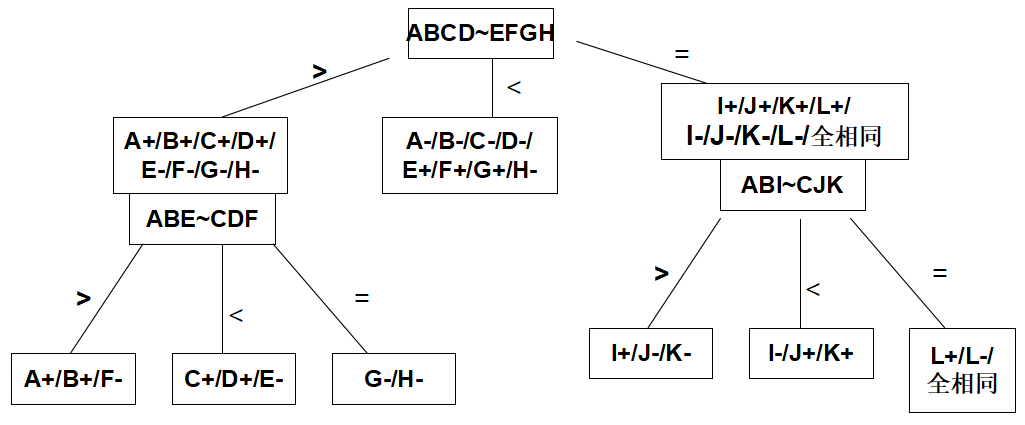
\includegraphics[scale=0.4]{判定硬币质量(决策树).png}
    \end{figure}
\end{enumerate}
\subsection{算法的概念}
\begin{definition}[算法]
    算法是\textbf{完成特定任务的有限指令集合}. 
    满足的标准为:
    \begin{enumerate}
        \item 输入:由\textbf{零个或多个外部量}作为算法输入.
        \item 输出:算法产生\textbf{至少一个量}作为输出.
        \item 确定性:组成算法的指令\textbf{清晰、无歧义}.
        \item 有限性:算法中每条指令的执行\textbf{次数、时间有限}.
        \item 可行性:每条指令均能用\textbf{有限的运算}完成.
    \end{enumerate}
\end{definition}
\begin{definition}[程序]
    程序是算法在某种程序设计语言下的具体实现,无需满足算法中的有限性(例如操作系统是无限循环).
\end{definition}
\begin{definition}[算法复杂性]
    算法复杂性是算法运行所需的计算机资源量. 
    进一步划分为两部分:所需的时间资源量称为\textbf{时间复杂性},所需的空间资源量称为\textbf{空间复杂性}.
\end{definition}
\begin{remark}
    \item 一般将数据规模记为$n$,将算法的输入实例记为$I$. 对于实例$I$,算法复杂性是关于$I$的函数,记为$C=F(I)$. 进一步划分,将算法的时间复杂性记为$T(I)$,空间复杂性记为$S(I)$.
    \item 用$\text{size}(I)$表示实例的规模,则$\text{size}(I) = n$表示规模为$n$的实例$I$.
    \item 由于时间复杂性与空间复杂性计算类似,主要考虑空间复杂性计算,往往空间复杂性低于时间复杂性(创建空间需要时间).
\end{remark}
\begin{definition}[3种时间复杂性]\ 
    \begin{enumerate}
        \item \textbf{最坏情况}下:$T_{max}(n) = \max\{T(I):\textrm{size}(I) = n\}$.
        \item \textbf{最好情况}下:$T_{min}(n) = \min\{T(I):\textrm{size}(I) = n\}$.
        \item \textbf{平均情况}下:$T_{avg}(n) = \sum_{\textrm{size}(I) = n}p(I)T(I)$,其中$p(I)$表示实例$I$出现的概率.
    \end{enumerate}
\end{definition}
\subsection{复杂性的渐进表示}
\begin{definition}[算法的渐近复杂性]
    设实例规模为$n$,函数$f(n)$表示算法的时间复杂性,若函数$g(n)$满足$f(n)/g(n)\to 1,\ (n\to\infty)$
    则称$g(n)$为算法的\textbf{渐近复杂性}.
\end{definition}
\begin{definition}[复杂性的渐近表示]设实例的规模为$n$,函数$f(n), g(n)>0$,其中$f(n)$表示算法的时间复杂性.
    \begin{enumerate}
        \item \textbf{渐进上界记号}:$\O(g(n)) = \{f(n):\exists c,n_0>0,s.t.\ f(n)/g(n)\leq c\ (\forall n \geq n_0)\}$.
        \item \textbf{渐近下界记号}:$\Omega(g(n)) = \{f(n):\exists c,n_0>0,s.t.\ f(n)/g(n)\geq c\ (\forall n \geq n_0)\}$.
        \item \textbf{紧渐进记号}:\del
        \begin{equation*}
            \Theta(g(n)) = \{f(n):\exists c_1,c_2,n_0>0,s.t.\ c_1\leq f(n)/g(n)\leq c_2\ (\forall n \geq n_0)\}.
        \end{equation*}
        \item \textbf{非紧上界记号}:$o(g(n)) = \{f(n): \forall \varepsilon > 0, \exists n_0 > 0,s.t.\ f(n)/g(n) < \varepsilon\ (\forall n \geq n_0)\}$.
        \item \textbf{非紧下界记号}:$\omega(g(n)) = \{f(n):\forall \varepsilon > 0, \exists n_0,s.t.\ f(n) / g(n) > \varepsilon\ (\forall n\geq n_0)\}$.
    \end{enumerate}
\end{definition}
\begin{remark}
    \item $\Theta(g(n)) = \O(g(n))\cap \Omega(g(n))$.
    \item $f(n)\in \O(g(n))$也记为$f(n) = \O(g(n))$,在等式中渐进记号表示该集合中的某个函数. 例$n^2+n = \O(n^2) = n^2 + \O(n)$.
    \item 互对称性:$f(n) = \O(g(n))\Leftrightarrow g(n) = \Omega(f(n))$,$f(n)= o(g(n))\Leftrightarrow g(n)= \omega(f(n))$.
    \item 易证渐进上界的性质:
    \begin{itemize}
        \item $\O(f(n)) + \O(g(n)) = \O(f(n)+g(n)) = \O(\max\{f(n),g(n)\})$.
        \item $\O(f(n))\O(g(n)) = \O(f(n)g(n))$.
        \item $\O(cf(n)) = \O(f(n))$.
        \item $g(n) = \O(f(n))\Rightarrow \O(f(n))+\O(g(n)) = \O(f(n))$
    \end{itemize}
\end{remark}
\begin{example}
    设$p(n) = \sum_{1\leq j\leq d}a_jn^j$,则$p(n) = \Theta(n^d)$.
\end{example}
\begin{solution}
    由于$a_d\leq \frac{p(n)}{n^d}\leq a_d+\sum_{1\leq j\leq d-1}a_jn^{j-d}\to a_d,\quad (n\to\infty)$,由左不等号知$p(n) = \Omega(n^d)$,右不等号知$p(n) = \O(n^d)$,于是$p(n) = \Theta(n^d)$.
\end{solution}
\subsection{算法复杂性分析方法}
\begin{definition}[程序步]
    程序步指语法上可测度的程序段,其执行时间为常量,与问题规模无关.(一般将非递归的语句视为一个程序步,通过分析程序步的个数,可以估计得到算法的时间复杂性.)
\end{definition}
\begin{example}
下面以插入排序为例,右侧注释为程序步的重复次数:
\begin{cppcode}
void insertion_sort(Type *a, int n)
{
    Type key;                        //   cost     times
    for (int i = 1; i < n; i++){     //    1        $n$   
        key=a[i];                    //    1        $n-1$ 
        int j=i-1;                   //    1        $n-1$ 
        while( j>=0 && a[j]>key ){   //    1        $\sum_{i=1}^{n-1}t_i$
            a[j+1]=a[j];             //    1        $\sum_{i=1}^{n-1}(t_i-1)$
            j--;                     //    1        $\sum_{i=1}^{n-1}(t_i-1)$
        }
        a[j+1]=key;                  //    1        $n-1$
    }
}
\end{cppcode}
则时间复杂性为$T(n) = n+3(n-1) + \sum_{i=1}^{n-1}t_i + 2\sum_{i=1}^{n-1}(t_i-1)$.
\begin{itemize}
    \item 最好情况下$t_i = 1$,则$T_{min}(n) = 5n-4 = \O(n)$.\add
    \item 最坏情况下$t_i = i+1$,则$T_{max}(n) = \frac{3}{2}n^2+\frac{7}{2}n-4=\O(n^2)$.
\end{itemize}
\end{example}
\begin{example}[堆构建的时间复杂度计算]
    假定对于一个有$n$个顶点的完全二叉树,当该树为满二叉树时需要筛选调整的次数最多,此时有$n=2^d-1$,其中$d=\lceil logn \rceil$.

    对于深度为$d$的满二叉树,第$k(k\geq 0)$层有$2^k$个节点,每个节点最多向下调整$d-k-1$次,最坏情况下,堆构建所需的比较次数为:
    \begin{equation*}
        T_{max}(n) = \sum_{k=0}^{d-1}2^k(d-k-1) =  (d-1)\sum_{k=0}^{d-1}2^k-\sum_{k=0}^{d-1}k2^k = 2^d-d-1 = \O(n)
    \end{equation*}
\end{example}

\section{递归与分治策略}
\subsection{递归算法}
\begin{definition}[递归算法、递归函数]
    直接或间接调用自身的算法称为\textbf{递归算法};用函数自身给出定义的函数称为\textbf{递归函数}.
\end{definition}
\begin{example}[全排列问题]
    用递归算法生成集合$R=\{r_1,\cdots, r_n\}$的全排列. 记$\text{perm}(R)$为集合$R$生成的全排列,$n = |R|$为$R$的基数,则$\text{perm}(R) = \begin{cases}
        \varnothing,&\quad R=\varnothing,\\
        \bigcup_{i=1}^n(r_i)\text{perm}(R-\{r_i\}),&\quad n\geq 1.
    \end{cases}$,其中$(r_i)\text{perm}(R)$表示$\text{perm}(R)$中每个排列加上前缀$(r_i)$得到的排列.
    \begin{cppcode}
void perm(char a[], int i, int n) {
    if (i == n) {
        printf("%s\n", a);
        return;
    }
    for (int j = i; j < n; j++) {
        swap(a[i], a[j]);
        perm(a, i+1, n);
        swap(a[i], a[j]);
    }
} 
int main() {
    perm(a, 0, n);
    return 0;
}
    \end{cppcode}
\end{example}
\begin{example}[正整数划分]
    将正整数$n$划分为一系列正整数之和:$n=n_1+\cdots+n_k$,$(n_1\geq n_2\geq \cdots\geq n_k)$,求划分的个数.
    
    考虑动态规划,令$f(n,m)$表示正整数$n$划分中的最大正整数$n_1$不超过$m$的划分个数,则问题转化为求解$f(n,n)$. 不难发现$f$有以下递归关系:
    \begin{equation*}
        \begin{cases}
            f(n,m) = f(n,n),&\quad n<m,\\
            f(n,m) = f(n-m, m)+f(n,m-1),&\quad n\geq m,\\
            f(0,m) = f(1,m) = f(n, 1) = 1&\quad \text{边值条件}.
        \end{cases}
    \end{equation*}
    第一行和第三行易于理解,第二行是因为将$f(n,m)$的全部划分分为两种,第一种$n_1=m$,对应的划分个数为$f(n-m,m)$个;第二种$n_1\neq m$,对应划分个数为$f(n,m-1)$.
    \begin{cppcode}
int f(int n, int m) {
    if (n == 0 || n == 1 || m == 1) return 1;
    if (n < m) return f(n, n);
    return f(n-m, m) + f(n, m-1);
}
int main() {
    cout << f(n, n);
    return 0;
}
    \end{cppcode}
\end{example}
\begin{example}[Hanoi塔问题]
设A,B,C是3个塔座. 开始时,在塔座A上有一叠共$n$个圆盘,这些圆盘自下而上,由大到小地叠在一起. 各圆盘从小到大编号为$1,2,\cdots,n$,现要求将塔座A上的这一叠圆盘移到塔座B上,并仍按同样顺序叠置. 在移动圆盘时应遵守以下移动规则:

规则1:每次只能移动$1$个圆盘;

规则2:任何时刻都不允许将大的圆盘压在较小的圆盘之上;

规则3:在满足移动规则1和2的前提下,可将圆盘移至A,B,C中任一塔座上.

Hanoi塔有一个抽象的理解方法:将大象放进冰箱一共三步,打开冰箱,放入大象,关上冰箱. 这说的是“放入冰箱”这件事,无论向冰箱里放任何物体,总是可以划分为这三个步骤. Hanoi塔问题同理,将A塔上的$n$个圆盘移动到B塔上,只有三步:
\begin{enumerate}
    \item 将A塔上$n-1$个圆盘移动到C塔上.
    \item 将A塔上最后一个圆盘移动到B塔上.
    \item 将C塔上$n-1$个圆盘移动到B塔上.
\end{enumerate}
而上述第一个步骤和第三个步骤,同样可以转化为三个步骤,只不过塔的编号会发生变化. 
令$\text{hanoi}(n,a,b,c)$表示将a塔中的$n$个圆盘移动到b塔上的方案(注:此处的a,b,c表示塔的编号),则
\begin{equation*}
    \text{hanoi}(n,a,b,c) = \begin{cases}
        1.\ \text{hanoi}(n-1,a,c,b),\\
        2.\ \text{将a塔上的圆盘移动到b塔上},\\
        3.\ \text{hanoi}(n-1,c,b,a),\\
    \end{cases}
\end{equation*}
设移动次数为$f(n)$,则也可得到次数的递推式$f(n) = 2f(n-1)+1,\ f(1) = 1$,解得$f(n) = 2^n-1$. 
于是算法的时间复杂度为$\O(2^n)$.
\begin{cppcode}
// 3个塔座,从塔座a上的所有圆盘移动到塔座b上的具体方案
void hanoi3(int n, char a='A', char b='B', char c='C') {
    if (!n) return;
    hanoi3(n-1, a, c, b);
    printf("%c->%c\n", a, b);     //  Output:
    hanoi3(n-1, c, b, a);         //  A->B
}                                 //  A->C
                                  //  B->C
int main() {                      //  A->B
    hanoi3(3);                    //  C->A
    return 0;                     //  C->B
}                                 //  A->B
\end{cppcode}
\textbf{拓展}:如果是4个塔座,编号为A,B,C,D,将A塔上的圆盘全部移动到B塔上,则也可类似上述方法求解,假设移动$m$个圆盘到备用塔D上,再将剩余的圆盘通过3个塔座A,B,C从A移动到B上.

\begin{equation*}
    \text{hanoi4}(n,a,b,c,d)=\begin{cases}
        1.\ \text{hanoi4}(n-m,a,d,b,c),\\
        2.\ \text{hanoi3}(m, a, b, c),\\
        3.\ \text{hanoi4}(n-m,d,b,a,c).\\
    \end{cases}
\end{equation*}
设移动次数为$g(n)$,则$f(n) = 2g(n-m)+f(m),\ g(0)=0$,设$k=n/m$,则$g(n) = (2^{m/k}-1)(2^k-1)$,可通过数值方式求解不同$n$
对应的$m$以达到$g(n)$的最小值. 于是递归算法的时间复杂度为$\O(2^{n/m})$.
\begin{cppcode}
void hanoi4(int n, int m, char a='A', char b='B', char c='C', char d='D') {
    if (n < m) {
        hanoi3(n, a, b, c);
        return;                             //  Output:
    }                                       //  A->D
    hanoi4(n-m, m, a, d, b, c);             //  A->B
    hanoi3(m, a, b, c);                     //  A->C
    hanoi4(n-m, m, d, b, a, c);             //  B->C
}                                           //  A->B
int main() {                                //  C->A
    hanoi4(4, 3);                           //  C->B
    return 0;                               //  A->B
}                                           //  D->B
\end{cppcode}
\end{example}
\begin{example}[递推求解-分治法]\label{example-division}
    设$a,b,c$为正整数,$a\geq 1, b>1,c>0$,$T(n)$满足如下递归方程,求$T(n)$的渐近表示.
    \begin{equation*}
        T(n) =\begin{cases}
            c,&\quad n=1,\\
            aT(n/b)+cn,&\quad n\geq 2.
        \end{cases}
    \end{equation*}

    令$k = \log_bn$,则$T(n) = aT(n/b)+c = a^2T(n/b^2)+ac+c = \cdots = a^kT(1)+cn(a^{k-1}+a^{k-2}+1) = a^k + cn\sum_{i=0}^{k-1}(a/b)^i$,分为三类讨论
    \begin{enumerate}
        \item $a=b$:$T(n) = n+cnk = n+cn\log_bn = \O(n\log_bn)$.
        \item $a>b$:$T(n) = a^k+cn\frac{(a/b)^k-1}{a/b-1} = \O(n^{\log_ba})$.
        \item $a<b$:$T(n) = n^{\log_ba}+cn\frac{1-(a/b)^k}{1-a/b}\leq n+\frac{bc}{b-a}n = \O(n)$
    \end{enumerate}
\end{example}
\begin{example}[推测验证]\label{example-linear}
    先推测递归方程的大$\O$估计,然后用归纳法证明. 举个例子:
    \begin{equation*}
        T(n) = \begin{cases}
            c_1,&\quad n\leq 6,\\
            T(n/2)+T(n/3)+c_2n,&\quad n > 6.
        \end{cases}
    \end{equation*}
    由于$n/2+n/3=5/6n < n$,所以猜测$T(n) = \O(n)$.
    
    当$n\leq 6$时,取$c = c_1,n_0=1$,则$\forall 1\leq n\leq 6$有$T(n)\leq c_1$成立.

    假设$n\leq k$时,$T(n) = O(n)$成立,
    则$\exists c > 0, n_0 > 0$使得$\forall n\geq n_0$有$T(n)\leq cn$.
    讨论$n\leq k+1$的情况,则$T(n)\leq c(n/2+n/3)+c_2n = (5/6c+c_2)n$,
    令$c = 5/6c+c_2$,则取$c = 6c_2$,有$T(n)\leq cn$.

    综上,取$c = \max\{c_1,6c_2\}$,则$n\geq 1$时,$T(n)\leq cn\Rightarrow T(n) = \O(n)$.

\end{example}
\subsection{分治策略}
分治法的基本思想是将规模为$n$的问题分解为$k$个规模为$n/m$的子问题,这些子问题相互独立且与原问题相同,
递归求解这些子问题,采用\textbf{自顶向下的计算方式},
然后将各个子问题的解合并得到原问题的解,假设合并所用时间为$f(n)$,
则分治法的时间复杂度有如下递推关系
\begin{equation*}
    T(n) = \begin{cases}
        \O(1),&\quad n=1,\\
        kT(n/m)+f(n),&\quad n > 1.
    \end{cases}
\end{equation*}
通过展开递推式,可以得到$T(n) = n^{\log_mk}+\sum_{j=0}^{\log_mn-1}k^jf(n/m^j)$,
\textbf{例}\ref{example-division}就是分治法的一个特例.

\subsubsection{二分法搜索}
给定已排好序的$n$个元素$a[0\cdots n-1]$,从中找出元素$x$的序号$i$,使得$a[i] = x$.

不妨令数组$a$中元素递增,二分法将$n$个元素分为两半进行查找,如果$x < a[n/2]$,则$x$一定在$a[0\cdots n/2]$中,只需在左半部继续搜索$x$即可;反之,$x$一定在$a[n/2\cdots n]$中,只需在右半部继续搜索$x$即可. 由于每次将规模减小一半,所以时间复杂度为$\O(\log n)$.
\begin{cppcode}
// 返回第一个的大于等于x的索引
int binary_search(int a[], int x, int n) {
    int l = 0, r = n-1;
    while (l < r) {
        int mid = (l + r) / 2;
        if (x > a[mid]) l = mid + 1;
        else r = mid - 1;
    }
    return r+1;
}
int main() {
    int a[] = {1, 2, 5, 8, 10}, x = 5, n = sizeof(a)/sizeof(int);
    printf("%d=a[%d]\n", x, binary_search(a, x, n));
    // 与algorithm库中lower_bound函数功能一致
    printf("%d=a[%d]", x, lower_bound(a, a+n, x)-a);
    return 0;
}
\end{cppcode}
\subsubsection{大整数乘法}
    当两个较大的整数进行相乘时,由于计算结果超出计算机硬件处理大小,无法在常数时间内完成计算,所以需要设计大整数乘法,用数组中来表示大整数的每一位.(这里以10进制为例,书上以2进制为例,本质相同)

    十进制下有两个长度为$n$的数字$x,y$,不妨令$n=2^k(k\geq 1)$,则可以将$x,y$划分为两段:
    \begin{equation*}
        x = 10^{n/2}a+b,\quad y=10^{n/2}c+d
    \end{equation*}
    于是
    \begin{align*}
        xy =&\ (10^{n/2}a+b)(10^{n/2}c+d) = 10^nac+10^{n/2}(ad+bc)+bd\\
        =&\ 10^nac+10^{n/2}((a+b)(c+d)-ac-bd)+bd.
    \end{align*}
    按照上述展开,计算规模为$n$的整数相乘,需要$3$次规模为$n/2$的整数乘法,$2$次位移
    ($10^n,10^{n/2}$表示将数字分别在数组中位移$n,n/2$个长度,用$0$填补空缺),$6$次加、减法,于是
    整数乘法的时间复杂度为
    \begin{eqnarray*}
        T(n) = \begin{cases}
            \O(1),&\quad n=1,\\
            3T(n/2)+\O(n),&\quad n>1.
        \end{cases}
    \end{eqnarray*}
    由\textbf{例}\ref{example-division}可知,$T(n) = \O(n^{\log_23}) \approx \O(n^{1.59})$,
    比直接做竖式乘法$\O(n^2)$有所提高. 不过需要额外实现大整数加减法,实现较为复杂,这里不提供代码了.
    \begin{remark}
        \item 大整数乘法最优做法为快速Fourier变换(FFT),时间复杂度为$\O(n\log n)$.
        大整数乘法本质上一维的离散卷积,可以通过转化为对应Fourier变换的点积,从而将卷积的复杂度降为$\O(n)$,
        再使用Fourier逆变换回去即可得到乘积结果. 
        而求解Fourier变换与逆变换就需要用到FFT,本质使用的也是分治的思想实现加速,
        时间复杂度为$\O(n\log n)$.
    \end{remark}
\subsubsection{Strassen矩阵乘法}
设$A,B$为两个$n\times n$矩阵,$C = AB$,由于$C$也是$n\times n$的矩阵,计算每个元素需要$\O(n)$次计算,
所以直接求解$C$的时间复杂度为$\O(n^3)$.

不妨令$n=2^k$,通过对$A,B,C$进行分块,每个矩阵划分为$4$个大小为$(n/2)\times (n/2)$的方阵:
\begin{equation*}
A={\begin{bmatrix}A_{11}&A_{12}\\A_{21}&A_{22}\end{bmatrix}},\quad 
B={\begin{bmatrix}B_{11}&B_{12}\\B_{21}&B_{22}\end{bmatrix}},\quad 
C={\begin{bmatrix}C_{11}&C_{12}\\C_{21}&C_{22}\end{bmatrix}},
\end{equation*}
于是
\begin{equation*}
{\begin{bmatrix}C_{11}&C_{12}\\C_{21}&C_{22}\end{bmatrix}}=
{\begin{bmatrix}
    A_{11}B_{11}+A_{12}B_{21}&A_{11}B_{12}+A_{12}B_{22}\\
    A_{21}B_{11}+A_{22}B_{21}&A_{21}B_{12}+A_{22}B_{22}
\end{bmatrix}}.
\end{equation*}
如果直接进行上述计算时间复杂度仍是$\O(n^3)$,但是可以通过定义新的矩阵从而降低矩阵乘法次数:(应该不用记忆这些$M_i$)
\begin{equation*}
{\begin{aligned}
    M_{1}&=A_{11}(B_{12}-B_{22});\\
    M_{2}&=(A_{11}+A_{12})B_{22};\\
    M_{3}&=(A_{22}+A_{21})B_{11};\\
    M_{4}&=A_{22}(B_{21}-B_{11});\\
    M_{5}&=(A_{11}+A_{22})(B_{11}+B_{22});\\
    M_{6}&=(A_{12}-A_{22})(B_{21}+B_{22}),\\
    M_{7}&=(A_{11}-A_{21})(B_{11}+B_{12});\\
\end{aligned}}
\end{equation*}
仅通过$7$次矩阵乘法,再通过加减法,可以得到
\begin{equation*}
{\begin{bmatrix}
    C_{11}&C_{12}\\
    C_{21}&C_{22}
\end{bmatrix}}=
{\begin{bmatrix}
    M_{5}+M_{4}-M_{2}+M_{6}&M_{1}+M_{2}\\
    M_{3}+M_{4}&M_{5}+M_{1}-M_{3}-M_{7}
\end{bmatrix}}.
\end{equation*}
矩阵加减法的事件复杂度为$\O(n^2)$,于是Strassen矩阵乘法的时间复杂度递推式为
\begin{equation*}
    T(n) = \begin{cases}
        \O(1),&\quad n=2,\\
        7T(n/2)+\O(n^2),&\quad n>2.
    \end{cases}
\end{equation*}
由\textbf{例}\ref{example-division}可知,$T(n) = \O(n^{\log_27})\approx \O(n^{2.81})$.
\begin{remark}
    \item 后面有很多基于Strassen算法的改进,现在矩阵乘法的理论最优复杂度为$\O(n^{2.37188})$
    \footnote{2022年10月最佳界限,来源:\url{https://en.wikipedia.org/wiki/Computational_complexity_of_matrix_multiplication}},
    但是这些优化算法在实践中没有价值,由于在$\O$符号后的常数过大,
    使得它们只适用于当前计算机无法存储的矩阵大小.
\end{remark}
\subsubsection{棋盘覆盖}
在一个$2^k\times 2^k$的方形棋盘中,有一个方格为特殊方格,请使用以下三种形态的L型骨牌将除去特殊方格外的棋牌全部填充满:
\begin{figure}[htbp]
    \centering
    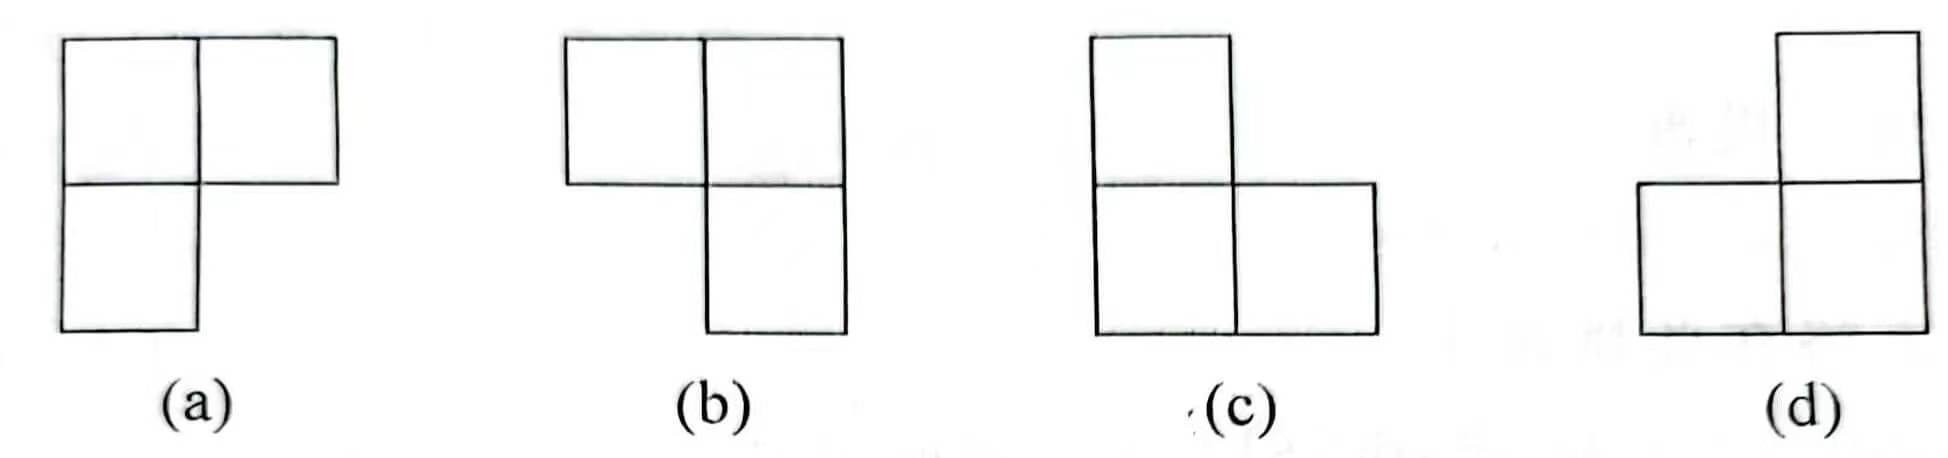
\includegraphics[scale=0.15]{four_L_dominos.jpg}
\end{figure}
在一个$2^k\times 2^k$的方形棋盘中,总共有$4^k-1$个待填充方格,由于$4^k-1 = 3\cdot 4^{k-1}+(4^{k-1}-1)$,
可通过归纳法证明$4^k-1$可以被$3$整除,所以如果能填充满,将使用$(4^k-1)/3$个骨牌.

使用分治法,每次将整个棋盘以“田”形状划分为$4$个大小为$2^{k-1}\times 2^{k-1}$的棋盘,如果特殊方格在左上区域,则在四块的中心处
填上$(d)$型骨牌,则原问题转化为左上区域中特殊方块位置不变,其他三个区域特殊方块为填入的骨牌位置. 如下图所示:
\begin{figure}[htbp]
    \centering
    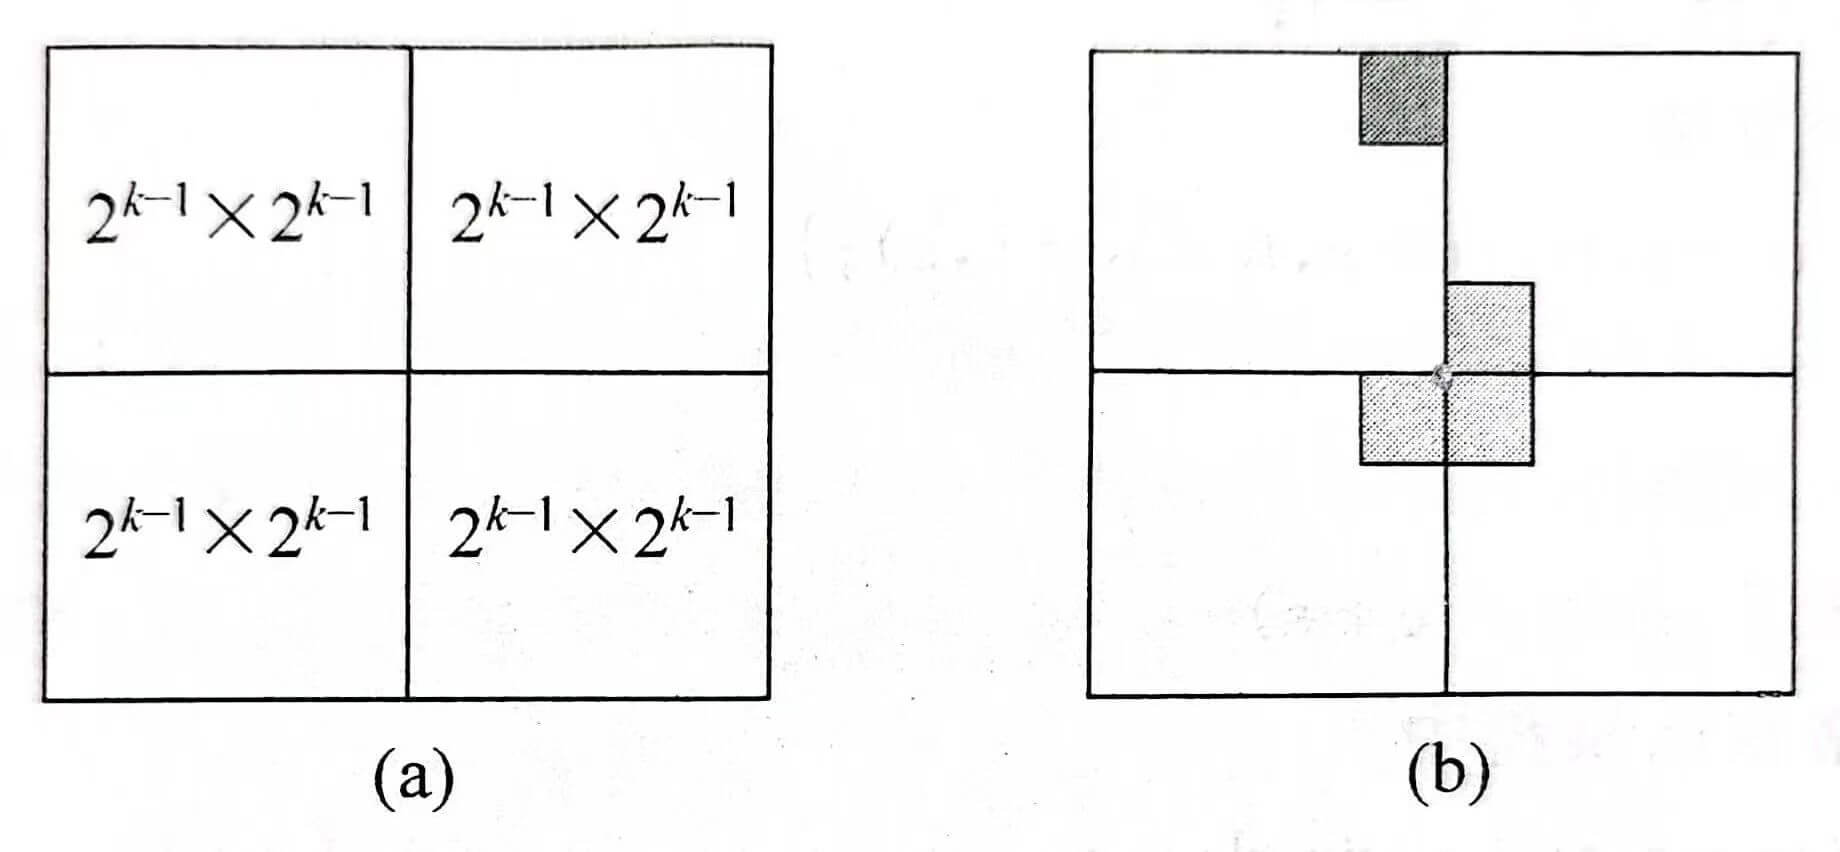
\includegraphics[scale=0.15]{board_division.jpg}
\end{figure}
当$k=0$时,填充结束. 上述算法已经说明填充方案一定存在,时间复杂度满足如下递归式:
\begin{equation*}
    T(k) = \begin{cases}
        \O(1),&\quad k=0,\\
        4T(k-1)+\O(1),&\quad k > 0.
    \end{cases}
\end{equation*}
则$T(k) = \O(4^k)$,与填充的总骨牌数目同阶,所以该算法是渐近意义下的最优算法.

\begin{cppcode}
const int N = (1<<10);
int total_dominos_counter;
char board[N][N];
void fill_board(int top_x, int top_y, int out_x, int out_y, int k) {
    if (k == 0) return;
    int domino_num = ++total_dominos_counter;
    int half_size = (1 << (k-1)), domino_counter = 0, area_index;
    int mid_x = top_x + half_size, mid_y = top_y + half_size;
    // 左上棋盘
    if (out_x < mid_x && out_y < mid_y) {
        area_index = 0;
        fill_board(top_x, top_y, out_x, out_y, k-1);
    } else {
        board[mid_x-1][mid_y-1] = domino_num;
        fill_board(top_x, top_y, mid_x-1, mid_y-1, k-1);
    }
    // 右上棋盘
    if (out_x < mid_x && out_y >= mid_y) {
        area_index = 1;
        fill_board(top_x, mid_y, out_x, out_y, k-1);
    } else {
        board[mid_x-1][mid_y] = domino_num;
        fill_board(top_x, mid_y, mid_x-1, mid_y, k-1);
    }
    // 左下棋盘
    if (out_x >= mid_x && out_y < mid_y) {
        area_index = 2;
        fill_board(mid_x, top_y, out_x, out_y, k-1);
    } else {
        board[mid_x][mid_y-1] = domino_num;
        fill_board(mid_x, top_y, mid_x, mid_y-1, k-1);
    }
    // 右下棋盘
    if (out_x >= mid_x && out_y >= mid_y) {
        area_index = 3;
        fill_board(mid_x, mid_y, out_x, out_y, k-1);
    } else {
        board[mid_x][mid_y] = domino_num;
        fill_board(mid_x, mid_y, mid_x, mid_y, k-1);
    }
}
void print_board(int k);  // 显示棋盘,略去
int main() {                            
    int out_x = 2, out_y = 3, k = 2;    //  Output:
    board[out_x][out_y] = 0;            //  2  2  3  3
    fill_board(0, 0, out_x, out_y, k);  //  2  1  1  3
    print_board(k);                     //  4  1  5  0
    return 0;                           //  4  4  5  5
}
\end{cppcode}
\subsubsection{合并排序与快速排序}
合并排序算法是利用分治法实现对$n$个元素进行排序的算法,基本思想为:将待排序的元素分为大小相同的2个子集合,分别对2个子集合进行排序,
最终将排序好的子集合合并.
\begin{cppcode}
const int N = 1e5;
int b[N];  // 临时数组
void merge(int a[], int left, int mid, int right) {
    int i = left, j = mid, k = 0;
    while (i < mid && j < right) {
        if (a[i] < a[j]) b[k++] = a[i++];
        else b[k++] = a[j++];
    }
    while (i < mid) b[k++] = a[i++];
    while (j < right) b[k++] = a[j++];
}
void merge_sort(int a[], int left, int right) {
    if (left + 1 == right) return;
    int mid = (left+right) / 2;
    merge_sort(a, left, mid);
    merge_sort(a, mid, right);
    merge(a, left, mid, right);
    memcpy(a+left, b, (right - left) * sizeof(int));  // 将数组b拷贝到a中
}
int main() {
    int a[] = {5, 9, 2, 4, 1, 3}, n = sizeof(a)/sizeof(int);
    merge_sort(a, 0, n);
    for (int i = 0; i < n; i++) printf("%d ", a[i]);
    // Output: 1 2 3 4 5 9
    return 0;
}
\end{cppcode}
函数\texttt{merge}和\texttt{memcpy}时间复杂度均为$\O(n)$,则合并排序时间复杂度满足如下递推式:
\begin{equation*}
    T(n) = \begin{cases}
        \O(1),&\quad n \leq 1,\\
        2T(n/2) + \O(n),&\quad n > 1.
    \end{cases}
\end{equation*}
由\textbf{例}\ref{example-division}可知$T(n) = \O(n\log n)$. 而且合并排序是稳定型排序算法.

快速排序是基于分治策略的另一个排序方法,对于子数组$a[l\cdots r]$主要分为两步:
\begin{enumerate}
    \item 基准元划分:从$a[l,\cdots r]$中随机选取基准元$x=a[p]$,以将全部大于等于$x$的元素移动到$x$的右侧,
    小于$x$的元素移动到$x$的左侧,最终$x$的索引记为$q$.
    \item 递归:进一步递归$a[l\cdots q-1]$和$a[q-1\cdots r]$.
\end{enumerate}
快排相对于合并排序的优点在于无需额外的数组进行合并,最终得到的数组就是结果. 但是快速排序是不稳定的,
最坏情况可能是每次选取子数组中最小的元素,时间复杂度满足:
\begin{equation*}
    T_{max}(n) = \begin{cases}
        \O(1),&\quad n \leq 1,\\
        T_{max}(n-1)+\O(n),&\quad n > 1.
    \end{cases}\Rightarrow T_{max}(n) = \O(n^2)
\end{equation*}
最优情况是和分治排序相同,每次都能选取子数组的中值,将子数组长度划分为原来的一半,
于是$T_{min}(n) = \O(n\log n)$. 所以随机选取划分基准,在数组元素各不相同的情况下,
可以期望每次划分结果是对称的.
\begin{cppcode}
int random_partition(int a[], int left, int right) {
    int base_index = rand() % (right - left) + left;
    int x = a[base_index];
    swap(a[left], a[base_index]);
    int i = left+1, j = right-1;
    while (true) {
        while (a[i] <= x && i < right) i++;
        while (a[j] >= x && j > left) j--;
        if (i >= j) break;
        swap(a[i], a[j]);
    }
    swap(a[left], a[j]);
    return j;
}
void quick_sort(int a[], int left, int right) {
    if (left + 1 >= right) return;
    int base_index = random_partition(a, left, right);
    quick_sort(a, left, base_index);
    quick_sort(a, base_index+1, right);
}
int main() {
    srand(time(NULL));  // 根据时间初始化随机种子
    int a[] = {5, 9, 2, 4, 1, 3}, n = sizeof(a)/sizeof(int);
    quick_sort(a, 0, n);
    for (int i = 0; i < n; i++) printf("%d ", a[i]);
    // Output: 1 2 3 4 5 9
    return 0;
}
\end{cppcode}
\subsubsection{线性时间选择}
给定$n$个元素的数组和整数$1\leq k\leq n$,要求找出$n$个元素中第$k$小的元素.

假设当前处理的序列为\cppinline{a[1,...,n]},具体思想就是找当前序列的\textbf{中位数的中位数}作为基准. 
设函数\cppinline{select(l,r,k)}表示求解\cppinline{a[l,...,r]}中第$k$小的元素.

具体做法:我们假设以$5$个元素作为一个小组,将原数组划分为$\lfloor n/5\rfloor$个模$5$的剩余类,
例如$n=17$,则划分后的结果为\cppinline{[*****|*****|*****|**]}
(\cppinline{*}表示数组中的元素,一共得到$3$个小组),
然后我们对每个小组中的元素使用冒泡排序,冒泡$3$次即可找到小组中的中位数,
我们将中位数标记为\cppinline{$}符号,则排序后数组为\cppinline{[**$**|**$**|**$**|**]}. 
然后我们将每个小组的中位数全部移动到整个数组的左侧,即\cppinline{[$$$**|*****|*****|**]},
于是我们已经获得了中位数序列,即数组中开头三个,为了求解中位数的中位数,
我们再递归调用\cppinline{select}函数. 
以上面例子为例,我们只需求解\cppinline{select(1,3,2)}从而求解\cppinline{[$$$]}中的中位数,
即可得到原数组的中位数的中位数.

获得中位数的中位数\cppinline{x}后,再以\cppinline{x}作为基准元素,
利用类似快排的划分函数\\
\cppinline{partition(l,r,x)}(只不过这次给定了基准元素\cppinline{x}),
从而对原数组左右划分,再判断我们要查询的第$k$大元素是在基准的左侧还是右侧,递归查找即可.

\textbf{注}:如果有存在多个重复基准元素\cppinline{x},
我们需要将划分后的\textbf{基准元素全部聚集在中间},
假设有$m$个重复基准元素,于是原数组最终应该划分为\cppinline{[00000|$$$$|11111]},
其中\cppinline{0}、\cppinline{1}分别表示小于、大于基准元素的值,
\cppinline{$}表示基准元素. 于是原数组被划分为三分,
如果当前第$k$大元素落在中间的区间中,则直接返回基准元素,否则判断第$k$大元素在左侧还是右侧,递归查找即可.

上述算法的关键就是找到了当前序列的中位数的中位数,从而每次划分为两半时,
基准元素左侧至少会有$\lfloor n/4\rfloor$个元素. 保证每次查找至少可以减少$\lfloor n/4\rfloor$的数量级.

时间复杂度分析,设对序列长度为$n$的序列调用\cppinline{select}函数需要$T(n)$的时间,
则查找中位数的中位数至多使用$T(n/5)$,使用基准$x$划分原数组,{}
两个数组中至多还有$3n/4$个元素,则进一步递归调用至多使用$T(3n/4)$时间. 综上,$T(n)$递推式为
\begin{equation*}
    T(n) = Cn+T(n/5)+T(3n/4),
\end{equation*}
常数$C$主要包含每个小组的冒泡排序、\cppinline{partition}、聚集基准元素所花的时间. 
由\textbf{例}\ref{example-linear}可知$T(n) = \O(n)$.
\section{动态规划}
\subsection{基本要素}
\begin{enumerate}
    \item \textbf{最优子结构}:问题的最优解包含子问题的最优解.
    \item \textbf{重叠子问题}:递归求解问题时,可能多次产生相同的子问题.
\end{enumerate}
而动态规划就是在假设子问题最优的前提下,自底向上构造出整个问题的最优解;对于每个相同的子问题,
动态规划会将其记录在数组中,当再次解此问题时直接常数时间查看结果即可.

\textbf{注}:同一问题可以有多种方式刻画它的最优子结构.
\subsection{矩阵连乘问题}
在计算矩阵连乘问题时,对矩阵不同位置加上括号会对整个计算量产生影响,但对结果没有影响,求出最小的计算量.

若一个$a\times b$的矩阵与$b\times c$的矩阵进行相乘,所需程序步为$abc$步. 假设两个矩阵维数分别为
$10\times 100, 100\times 5, 5\times 50$若按照$(A_1A_2)A_3$次序计算,需要$10\times 100\times 5 +
10\times 5\times 50 = 7500$,如果按照$A_1(A_2A_3)$次序计算,需要
$10\times 5\times 50+10\times 100\times 50 = 75000$次计算,速度降低很多.

考虑动态规划,设定状态:$f(l,r)$表示合并左开右闭区间$[l,r)$中全部矩阵所需的最少次数,从中间选择切分点$k$,
则可以通过切分点左右两侧矩阵合并得到当前$[l,r)$全部矩阵方案,从中选取最少的即可.
\begin{equation*}
    f(l,r)=\begin{cases}
        0,&\quad l+1 = r,\\
        \min_{l < k < r}\{f(l, k) + f(k, r) + row[k]\times row[l]\times row[r]\},\quad l+1<r,
    \end{cases}
\end{equation*}
其中$row[i]$表示第$i$的矩阵的行数,最后一个矩阵的列数由$row[n+1]$表示.
\begin{cppcode}
const int N = 1e3;
const int INF = 0x3f3f3f3f;
int n = 6;
int dp[N][N], row[N] = {30, 35, 15, 5, 10, 20, 25};
int solve(int l, int r) {
    if (dp[l][r] != INF) return dp[l][r];
    for (int k = l+1; k < r; k++)
        dp[l][r] = min(dp[l][r], solve(l, k)+solve(k, r)+row[l]*row[k]*row[r]);
    return dp[l][r];
}
int main() {
    memset(dp, 0x3f, sizeof(dp));  // 初始化为极大值INF
    for (int i = 0; i < n; i++) dp[i][i+1] = 0;
    printf("%d\n", solve(0, n));  // Output: 15125
    return 0;
}
\end{cppcode}
\subsection{最长公共子序列}
对于两个长度为$n$的序列$a=\{a_1,\cdots,a_n\},b=\{b_1,\cdots, b_m\}$,子序列指的是将原序列中删去
若干个元素后得到的序列,例如$\{a_1,a_3\}$就是序列$a$的子序列. 求序列$a,b$的最长公共子序列长度.

设$f(i,j)$表示序列$\{a_1,\cdots, a_i\}$与序列$\{b_1,\cdots, b_j\}$的最长公共子序列长度,
则$f(n, m)$即为序列$a,b$的最长公共子序列长度,
且$f(i,j)$满足以下递推关系式:
\begin{equation*}
    f(i,j) =  \begin{cases}
        0,&\quad i=0,j=0,\\
        f(i-1,j-1)+1,&\quad a_i=b_j,\\
        \max\{f(i-1,j),f(i,j-1)\},&\quad a_i\neq b_j.
    \end{cases}
\end{equation*}
如果两个序列中最后一个元素相同,则直接在$f(i-1,j-1)$的最长公共子序列末尾加上$a_i$即可得到$f(i,j)$的
最长公共子序列;
否则$f(i,j)$的最长子序列一定和$f(i-1,j)$或者$f(i,j-1)$的最长子序列相同.
\subsection{电路布线(最大不交子集)}
设总共有$n$个二元组,$\pi$为序列$1,\cdots, n$的一个排列,二元组集合为$\text{Nets}=\{(t,\pi(t)):1\leq t\leq \pi(t)\}$,
定义二元组$(i,\pi(i))$与$(j,\pi(j))$相交,当且仅当,$i < j$且$\pi(i) > \pi(j)$. 求$\text{Nets}$的最大不交子集大小.

设$f(i, j)$表示$N=\{(t, \pi(t)):t\leq i,\pi(t)\leq j\}$的最大不交子集大小,
则$f(n,n)$为$\text{Nets}$的最大不交子集大小,且$f(i,j)$满足一下递推关系:
\begin{align*}
    f(i, j) =&\ \begin{cases}
        f(i-1, j),&\quad j < \pi(i),\\
        \max\{f(i-1,j), f(i-1, \pi(i)-1)+1\},&\quad j \geq \pi(i).
    \end{cases}\\
    \text{初始值: }f(1, j) =&\ \begin{cases}
        0, &\quad j < \pi(1),\\
        1, &\quad j \geq \pi(1).
    \end{cases}
\end{align*}
对于$f(i,j)$考虑是否将$(i,\pi(i))$纳入当前的最大不交子集,如果将其加入,则必须满足$j\geq \pi(i)$的前提,
并将其并入$f(i-1,\pi(i)-1)$的最大不交子集;或者,不加入$(i,\pi(i))$直接从$f(i-1,j)$转移得到.
\subsection{流水线调度}
设有$n$个任务需要在两台机器$M_1,M_2$上完成,第$i$个作业需要先在$M_1$上加工$a_i$小时,然后在$M_2$上加工
$b_i$小时,请问如何调度任务处理顺序,使得完成所有作业的总时间最小?

该问题解决方案有动态规划$\O(n^2)$和基于Johnson法则的排序算法$\O(n\log n)$. 通过动态规划方法可以推出
Johnson法则,然后证明Johnson法则具有传递性,则可以使用排序算法对任务顺序按照Johnson法则进行排序.

设$f(S, t)$表示距离$M_2$空闲还差$t$小时前提下,完成任务集合$S$中全部作业所需的最少时间,则完成全部作业
所需的最少时间为$f(N, 0)$,其中$N = \{1,2,\cdots,n\}$,且$f(S,t)$满足一下递推式:
\begin{equation*}
    f(S, t) = \min_{i\in S}\{a_i + f(S-\{i\}, b_i+\max\{t-a_i,0\})\},
\end{equation*}
其中$\max\{t-a_i, 0\}$表示先完成第$i$个任务在$M_1$上的工序后,$M_2$机器剩余的时间.

下面考虑最优排列$\pi$中两个相邻的编号$i=\pi(k),j=\pi(k+1)$,则由上述转移方程可知,
先加工第$i$个任务,再加工第$j$个任务,加工完第$i$个任务后,距离$M_2$空闲所需的时间为:
\begin{align*}
    t_{ij} =&\ b_i + \max\{b_i+\max\{t-a_i,0\}-a_j,0\}\\
    =&\ b_j+b_i-a_j+\max\{\max\{t-a_i,0\},a_j-b_i\}\\
    =&\ b_j+b_i-a_j+\max\{t-a_i,a_j-b_i,0\}\\
    =&\ b_j+b_i + \max\{t-a_i-a_j, -b_i, -a_j\}.
\end{align*}
假设我们将$i,j$任务交换加工顺序,加工完第$j$个任务后,距离$M_2$空闲所需的时间为:
\begin{equation*}
    t_{ji} = b_j+b_i + \max\{t-a_i-a_j, -b_j, -a_i\}
\end{equation*}
所以要求$t_{ij} \leq t_{ji}$,等价于
\begin{equation*}
    \max\{-b_i, -a_j\}\geq \max\{-b_j, -a_i\}\iff \min\{b_i, a_j\}\leq \min\{b_j, a_i\}.
\end{equation*}
上式被称为Johnson法则,可以通过枚举法证明Johnson法则满足传递性,即如果$(a_i,b_i)$与$(a_j,b_j)$
满足Johnson法则,$(a_j,b_j)$与$(a_k,b_k)$满足Johnson法则,则$(a_i,b_i)$与$(a_k,b_k)$也满足Johnson法则,
又由于最优调度序列等价于$\forall 1\leq i < j\leq n$,$(a_i,b_i)$与$(a_j,b_j)$满足Johnson法则.

所以,只需对二元组序列$\{(a_i,b_i):1\leq i\leq n\}$按照Johnson法则进行排序即可得到最优序列,时间复杂度为
$\O(n\log n)$.
\del
\subsection{01背包问题}\del
\subsubsection{动态规划方程}
总共有$n$个物品,其中第$i$个物品的价值为$v_i$,重量为$w_i$,现有一个最多容纳重量为$C$的背包,
求放入背包物品的总价值的最大值.

设$f(i,j)$表示$i,i+1,\cdots,n$个物品,放入大小为$j$的背包所产生的最大价值,则全部物品放入大小为$C$的背包
能产生的最大价值为$f(n,C)$,且$f(i,j)$满足一下递推式:
\begin{equation*}
    \forall 1\leq i < n,\quad f(i,j) = \begin{cases}
        f(i+1,j),&\quad j < w_i,\\
        \max\{f(i+1,j),v_i+f(i+1,j-w_i)\},&\quad j\geq w_i.
    \end{cases}
\end{equation*}
初始化条件为
$f(n, j) = \begin{cases}
    0, &\quad j < w_n,\\
    v_n,&\quad j \geq w_n.
\end{cases}$

动态规划思路与电路布线类似,每次考虑第$i$个物品是否放入到背包中,如果空间允许的前提下$j\geq w_i$,
则放入背包后剩余大小为$j-w_i$,可以从$f(i-1,j-w_i)$的最大价值背包中放入第$i$个物品;或者,
不放入第$i$个物品,则直接从$f(i-1,j)$进行转移. 时间复杂度为$\O(cn)$.
\begin{cppcode}
const int N = 1001;
int dp[N][N];
int knapsack(int n, int c, int v[], int w[]) {
    for (int j = w[n]; j <= c; j++) dp[n][j] = v[n];  // 初始化边界条件
    for (int i = n-1; i >= 1; i--) {
        for (int j = 0; j <= c; j++) {
            dp[i][j] = dp[i+1][j];  // 从上个状态转移过来
            if (j >= w[i])  // 考虑是否加入第i个物品
                dp[i][j] = max(dp[i][j], v[i] + dp[i+1][j-w[i]]);
        }
    }
    return dp[1][c];  // 返回最优解
}
\end{cppcode}
\del\del
\subsubsection{跳跃点集合合并}
基于上述动态规划方程的基础上,考虑一种和背包大小无关的时间复杂度.

举个例子:$n=5,c=10,w = \{2,2,6,5,4\},v=\{6,3,5,4,6\}$,则$i=5$时,由递推初始条件可知\del
\begin{equation*}
    f(5, j) = \begin{cases}
        0,&\quad j < 4,\\
        6,&\quad j\geq 4.
    \end{cases}
\end{equation*}
固定$i$将$f(i,j)$视为$j$的函数,记$f_i(j) := f(i,j)$,则由$f(i,j)$的定义可知,
$f_i(j),\ (1\leq i\leq n)$是关于$j$的阶梯状单调不减函数,$f_5(j)$的跳跃点为$\{(0,0), (4,6)\}$. 

我们给出跳跃点的定义:若$(j, f_i(j)),\ (j\geq 1)$是跳跃点,当且仅当,
$f_i(j)\neq f_i(j-1)$,并将$(0,0)$视为跳跃点. 

设$P_i$是$f_i(j)$的全部跳跃点集合,则
\begin{equation*}
    P_i = \{(j, f_i(j)):f_i(j)\neq f_i(j-1), j\geq 1\}\cup\{(0, 0)\}
\end{equation*}
由动态规划递推式$f(i,j) = \max\{f(i+1,j),f(i+1,j-w_i)+v_i\}$可知,$P_i$也可递推得到,初始化$P_{n+1} = \{(0,0)\}$. 

记函数$f(i+1,j-w_i)+v_i$的跳跃点为$Q_{i+1}$,则有$P_i\subset P_{i+1}\cup Q_{i+1}$,
不难发现$Q_{n+1}$可以由$P_{n+1}$中每个向量加上$(w_i,v_i)$直接得到(注意当前重量$j$不能超过背包大小$c$),即
\begin{equation*}
    Q_{i+1} = \{(j+w_i,f_{i+1}(j)+v_i):(j,f_{i+1}(j)\in P_{i+1}),\ j+w_i\leq c\} =: P_{i+1}\oplus (w_i,v_i)
\end{equation*}

由于在$P_{i+1}\cup Q_{i+1}$中可能出现$(a,b),(c,d)$满足$a\leq c,\ b>d$的情况,将$(c,d)$点称为受控跳跃点,
将$P_{i+1}\cup Q_{i+1}$中全部受控跳跃点删去即可获得$P_i$. 于是就可以通过递推得到$P_n,P_{n-1},\cdots,P_1$,
最终$P_1$中最后一项$j_{max} = \max_{(j, f_1(j))\in P_1}j$对应的$f_1(j_{max})$就是问题的解.

还是举这个例子:$n=5,c=10,w = \{2,2,6,5,4\},v=\{6,3,5,4,6\}$,初始化$P_6 = \{(0,0)\}$,
向其中每个向量加上向量$(w_5,v_5)=(4,6)$得到$Q_6 =P_6\oplus(w_5,v_5) = \{(4,6)\}$,求并集$P_6\cup Q_6$然后看是否有受控跳跃点,
如果有将其删去就可得到$P_5$,这里没有,就直接得到$P_5 = \{(0,0),(4,6)\}$;\del
\begin{align*}
    Q_5 =&\ P_5 \oplus (w_4,v_4) =  \{(5, 4), (9, 10)\},\\
    P_4 =&\ \{(0, 0), (4, 6), (9, 10)\},\quad\text{删去受控跳跃点}(5,4),\\
    Q_4 =&\ P_5 \oplus (w_3,v_3) =  \{(6,5),(10,11)\},\\
    P_3 =&\ \{(0, 0), (4, 6), (9, 10), (10, 11)\},\quad\text{删去受控跳跃点}(6,5),\\
    Q_3 =&\ P_5 \oplus (w_2,v_2) =  \{(2, 3), (6, 9)\},\\
    P_2 =&\ \{(0, 0), (2,3), (4, 6), (6, 9), (9, 10), (10, 11)\},\\
    Q_2 =&\ P_5 \oplus (w_1,v_1) =  \{(2,6),(4,9),(6,12),(8,15)\},\\
    P_1 =&\ \{(0, 0), (2,6), (4, 9), (6,12), (8, 15)\},\quad\text{删去受控跳跃点}(2,3),(4,6),(6,9),(9,10),(10,11),\\
\end{align*}
选择$P_1$中最后一项$(8,15)$,第二分量表示$f(1,c) = f(1,8) = 15$,所以问题的最优解为$15$.

\textit{该算法的时间复杂度为$\O(2^n)$,本质上和直接暴力枚举每个物品选与不选速度相同,但是由于可以用于出考试题.}
\section{贪心算法}
\subsection{贪心算法与动态规划}
贪心算法:通过每个局部最优解可直接得到全局最优解.

动态规划:通过将原问题划分为多个子问题,求解每个子问题,从而得到全局最优解.

共同之处:两者均需要问题具有\textbf{最优子结构,即问题的最优解包含子问题的最优解}. \\
\textit{动态规划算法通常以\textbf{自底向上}的方式解各子问题,而贪心算法则通常以\textbf{自顶向下}的方式进行.}

\subsection{背包问题(非01背包)}
不同于01背包,背包问题中,第$i$个物品的重量为$w_i$,价值为$v_i$,价值均匀分布在重量上,
可以选择物品$i$的一部分,无需将整个物品全部装入背包,如何选择装入背包的问题使得总价值最大?

由于将部分物品装入,所以最终背包一定可以被填满,利用贪心的思想,容易想到,应该
优先填入当前单位重量价值最高的物品,直至背包填满. 所以,做法就是先计算每个物品的单位重量价值,
然后从大到小排序,从单位价值由高到低选择物品填入背包,
最后无法完全填入背包的物品,将背包剩余部分填满即可.
\subsection{活动安排}
设有$n$个活动在同一个场地举行,第$i$个活动占用的时间段为$[a_i,b_i)$,要求不能有两个活动
在同一时间举行,求最多能举行多少场活动?

将全部活动对$b_i$从小到大排序,从第一个活动依次贪心地进行选择,活动$i$的开始时间$a_i\geq $
当前最后一个活动的结束时间,则选择该活动.

由于每个活动的重要性相同,所以每个活动为后续活动提供更多的时间,才能达到局部最优,如果活动的
重要性不同,就需要考虑使用动态规划求解了.

\subsection{Huffman编码}
$n$个符号,第$i$个符号出现的频率为$f_i$,使用二进制\textbf{前缀码}对符号进行编码,
第$i$的符号编码的码长记为$l_i$,则\textbf{平均码长}定义为$\sum_{1\leq i\leq n}f_i\cdot l_i$,
称最小平均码长对应的编码为Huffman编码. 

\textbf{前缀码}:任一编码不能是其他编码的前缀. 通过建立二叉树,从树根到每个叶子节点对应的路径
可以确定叶子节点的二进制前缀码,向左儿子移动路径记为$0$,右儿子移动路径记为$1$.

\textbf{建立Huffman编码树算法}:首先将每个符号视为独立的节点,节点权重为对应的频率,每次将权重最小的两个节点
合并为一个新的节点,新节点的权重为两个节点的权重之和,重复上述操作$n-1$次,最终只剩下一个节点停止. 
这样就能得到一棵二叉树,即为所求的Huffman编码树,每个符号均在叶子节点上,从根节点到叶子节点的路径对应了
该叶子上符号的编码.

\textbf{时间复杂度}:Huffman树中选择最小权重过程可使用小根堆实现,从而时间复杂度为$\O(n\log n)$.

\subsection{单源最短路经(Dijkstra)}
\textbf{Dijkstra算法为贪心算法}. 设非负权图$G=(V,E)$,其中$V$为顶点集,$E$为边集,给定顶点$r\in V$
为源点,求从$r$到$V-\{r\}$中每个点的最短路径,该问题称为单源最短路径问题.

\textbf{Dijkstra算法}:设顶点集合$S$为已知最短路径的顶点,初始时$S = \{r\}$,并用$r$对其周围顶点的最短路径进行
更新,我们将其称为“扩展”,每次从$V-S$中选择当前路径长度最小的顶点$u$进行扩展,并将$u$加入到$S$中,
直到$S=V$停止算法.

\textbf{时间复杂度}:Dijkstra算法中选择最小长度的顶点可通过小根堆实现,从而时间复杂度为$\O(n\log n)$.

\subsection{最小生成树(Prim,Kruskal)}
设$G=(V,E)$为无向连通带权图(也称为\textbf{网络}),若$G$的子图$G'$是包含$G$的所有顶点的树,
则称$G'$为$G$的\textbf{生成树}. $G'$的所有边权之和称为该生成树的\textbf{耗费},
$G$的全部生成树中最小耗费的,称为\textbf{最小生成树}.

设$V = \{1,2,\cdots, n\}$,若存在连接$i,j\in V$顶点的边,则$c(i,j)$表示连接顶点$i,j$边的权重.

\textbf{Prim算法}\footnote[1]{该书上的Prim算法与刁在筠的《运筹学》中讲的有所不同,算法设计课本讲的应该是正确算法.}:
令$S = \{1\}$,选择$i\in S,j\in V-S$
且$c(i,j)$最小的边,则将$j$加入$S$中,并连接$i,j$节点,重复上述操作,直到$S=V$停止算法,
即可得到最小生成树.

\textbf{Kruskal算法}:对全部的边按照边权值进行排序,先将原图中所有的边删去,即每个点均为孤立的连通分支. 
依边权从小到大一次遍历所有边,设当前遍历到的边为$e=(i,j)$,若顶点$i,j$不连通(即连接$i,j$不会产生环),
则连接$i,j$,依次处理完全部的边,即可得到最小生成树.

\textbf{时间复杂度}:Prim算法每次需要,考虑两个集合中的全部点对,记录每次$V-S$中每个节点到$S$的最短距离,
再在$V-S$选出最短距离的节点加入到$S$中,时间复杂度为$\O(n^2)$;
Kruskal算法只需对边权进行一次排序,再使用并查集判断两个顶点是否在同一个集合中,
时间复杂度为$\O(m\log m)$,其中$m$为图中边的个数;
当$m = \Theta(n^2)$时,Prim算法更优;当$m = o(n^2)$时,Kruskal算法更优.

\section{回溯法}
\subsection{概念}
\textbf{问题的解向量}:回溯法将一个问题的解表示为一个$n$元式$(x_1,\cdots, x_n)$的形式.

\textbf{显约束}:对分量$x_i$的取值限定.

\textbf{隐约束}:为满足问题的解而对不同分量之间施加的约束.

\textbf{约束条件}:显约束与隐约束共同组成约束条件.

\textbf{解空间}:对于问题的一个实例,解向量满足显示约束条件的所有多元组,构成该实例的一个解空间.

\subsection{生成问题状态的方法}
\textbf{生成问题状态两种方法}:问题状态的生成是从开始结点开始,在搜索过程中不断扩展已有结点完成. 
生成问题状态有两种本质上不同的方法:\textbf{深度优先生成方法}和\textbf{广度优先生成方法}
(与图搜索中的深度优先搜索和广度优先搜索相同).

\textbf{扩展结点}:一个正在生成子结点的结点.

\textbf{活结点}:已由其他节点生成的结点但为其子结点还未全部生成.

\textbf{死结点}:所有子结点已全部生成的结点.

\textbf{回溯法定义}:为避免生成不能产生最优解的问题状态,要用限界函数处死不能产生最优解的活结点. 
以减少问题的计算量. \textbf{具有限界函数的深度优先生成法}称为回溯法.

\subsection{回溯法基本思想}
\begin{enumerate}
    \item 针对给定的问题,定义问题的解空间;
    \item 确定易于搜索的解空间结构;
    \item 以深度优先搜索方式搜索解空间,并在搜索过程中用\textbf{剪枝函数}避免无效搜索.
\end{enumerate}
常用\textbf{剪枝函数}有以下两个:
\begin{itemize}
    \item \textbf{约束函数}是检测约束条件的函数,可以剪去不满足约束条件的子树;(保证解的可行性)
    \item \textbf{限界函数}是计算当前结点能够获得的最优界限,可以剪去必定得不到最优解的子树. 
    (使算法在子树中可能获得最优解)
\end{itemize}
\textbf{注记}:回溯法的本质就是\textbf{在暴力枚举问题的全部解的基础上用剪枝函数进行了筛选},
尽可能降低时间复杂度到可容忍的范围内. 
暴力枚举的方法有递归和非递归两种,枚举问题有枚举子集和枚举全排列两种经典问题.

\subsection{回溯法的结构}
\subsubsection{回溯法实现方法}
回溯法的实现一般有两种实现方式:\textbf{递归回溯}和\textbf{迭代回溯(非递归形式)}.

\textbf{递归回溯}:一般情况下使用递归方式实现回溯法,递归函数形式如下
\begin{cppcode}
void backtrack(int deep) {
    if (deep > n) output(track);
    else {  // start, end为显约束
        for (int i = start(n, deep); i <= end(n, deep); i++) {
            track[deep] = state(i);
            if (constraint(n, track) && bound(n, track))  // constraint为隐约束
                backtrack(deep + 1);
        }
    }
}
\end{cppcode}
其中\texttt{deep}表示递归深度,\texttt{n}表示递归最大深度,\texttt{track}为当前递归得到的可行解(状态序列),
\texttt{output}表示记录或输出当前得到的可行解,\texttt{start(n, deep)}和\texttt{end(n, deep)}
表示当前扩展结点处未搜索过的子树的起始编号和终止编号,\texttt{state(i)}表示当前扩展结点对应的状态可选值.
\texttt{constraint}和\texttt{bound}分别表示当前状态序列
的约束函数和限界函数. 若\texttt{constraint}返回为假,则当前的状态序列不满足约束条件,舍去;
若\texttt{bound}返回为假,则当前状态序列继续向下迭代无法产生最优解,舍去;
将\texttt{constraint}和\texttt{bound}两类函数统称为\textbf{剪枝函数}.

下面是非递归版本的回溯法,称为\textbf{迭代法}:
\begin{cppcode}
void iterative_backtrack() {
    int deep = 1;
    while (deep > 0) {
        if (start(n, deep) <=  end(n, deep)) {
            for (int i = start(n, deep); i <= end(n, deep); i++) {
                track[deep] = state(i);
                if (constraint(n, track) && bound(n, track)) {
                    if (deep > n) output(track);
                    else deep++;
                }
            }
        } else deep--;
    }
}
\end{cppcode}
在上述迭代算法中,除了每次需要重新计算当前层的\texttt{start(n, deep),end(n,deep)}外,
其他部分与递归法没有较大的区别.(本质是通过模拟栈结构实现非递归,\texttt{deep}为栈的层数)

\textbf{空间复杂度}:回溯法在搜索过程中动态产生问题的解空间,算法只需保存从根结点到当前扩充结点的路径,
若搜索树的高度为\texttt{h(n)},则回溯法的计算空间为$\O(h(n))$(只需一个大小为$h(n)$的堆栈即可),
如果需要显示存储整个解空间(完整地存储整个搜索树),则需要$\O(2^{h(n)})$或$\O(h(n)!)$空间大小.

\subsubsection{两种经典解空间树}
\textbf{子集树}:给定大小为$n$的集合$S$,需要找出$S$的满足某种条件的子集合,相应的解空间称为\textbf{子集树}. 
由于$S$中每个元素具有选与不选两种状态,所以搜索树为二叉树,总结点数目为$2^{n+1}-1$,
有$2^n$个叶结点,所需的时间复杂度为$\Omega(2^n)$.

子集树的一般算法可描述为以下形式:
\begin{cppcode}
void backtrack_subset(int deep) {
    if (deep > n) output(track);
    else {
        for (int i = 0; i <= 1; i++) {  // 二叉树,第deep个元素选与不选
            track[deep] = i;
            if (constraint(track) && bound(track))
                backtrack_subset(deep + 1);
        }
    }
}
\end{cppcode}
\textbf{注}:若题目要求画出子集树时,根据书本习惯,一般将左儿子视为“选”,右儿子视为“不选”,
如下图\ref{figure-子集树}所示.
\begin{figure}[htbp]
    \centering
    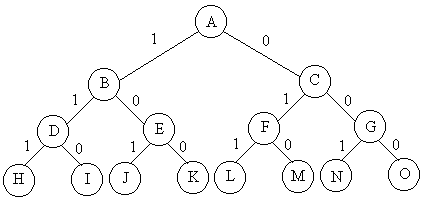
\includegraphics[scale=0.8]{01背包用完全二叉树表示解空间.png}
    \caption{用完全二叉树表示01背包问题的解空间}
    \label{figure-子集树}
\end{figure}

\textbf{排列树}:当问题为确定$n$个元素具有某种排列性质时,相应的解空间树称为\textbf{排列树}. 
排列树有$n!$个叶结点,所需的时间复杂度为$\Omega(n!)$.

排列树的一般算法可描述为以下形式:
\begin{cppcode}
void backtrack_permutation(int deep) {
    if (deep > n) output(track);
    else {
        for (int i = deep; i <= n; i++) {
            swap(track[deep], track[i]);
            if (constraint(track) && bound(track))
                backtrack_permutation(deep + 1);
            swap(track[deep], track[i]);
        }
    }
}
\end{cppcode}
在使用\texttt{backtrack\_permutation}前,先将搜索状态初始化为单位排列$(1,2,\cdots, n)$.
\del
\subsection{回溯法应用}
\del
\subsubsection{n皇后问题}
在$n\times n$的棋盘上放置$n$个彼此不受到攻击的皇后,两个皇后不收到攻击,当且仅当,不放在同一行或同一列
或统一斜线上.

设第$i$行皇后放置的位置为第$x_i$列,则解向量为$(x_1,\cdots, x_n)$,显约束为$x_i=1,2,\cdots, n$,隐约束
为 $\forall 1\leq i, j\leq n,\ i\neq j$满足
\begin{enumerate}
    \item $x_i\neq x_j$.
    \item 不在同一斜线上,$x_i-i\neq y_j-j$且$x_i+i\neq y_j+j$.
\end{enumerate}
\begin{cppcode}
const int N = 100;
int n=8, sum;
bool column[N], diag1[N], diag2[N];
void n_queens(int i) {
    if (i >= n) sum++;
    else {
        for (int j = 0; j < n; j++) {
            if (diag1[i+j] || diag2[i-j+n] || column[j])
                continue;
            diag1[i+j] = diag2[i-j+n] = column[j] = 1;
            n_queens(i+1);
            diag1[i+j] = diag2[i-j+n] = column[j] = 0;
        }
    }
}
int main() {
    n_queens(0);
    printf("%d\n", sum);
    return 0;
}
\end{cppcode}
\subsubsection{最大团问题}
设无向图$G = (V,E)$,$U\subset V$.
\textbf{完全子图}:$\forall u, v \in U$有$(u,v)\in E$,则$U$是$G$的完全子图.
\textbf{团}:$G$的完全子图$U$是$G$的团,当且仅当,$U$不包含于$G$更大的完全子图中.
\textbf{最大团}:$G$中顶点数最多的团.
\textbf{空子图}:$\forall u,v\in U$有$(u,v)\notin E$,则$u$为$G$的空子图.
\textbf{独立集}:$G$的空子图$U$为$G$的独立集,当且仅当,$U$不包含于$G$更大的独立集中.
\textbf{最大独立集}:$G$中顶点数最多的独立集.
\textbf{补图}:$G' = (V,E')$,$E' = \{(u,v):u,v\in V, (u,v)\notin E\}$,则$G'$称为$G$的补图.
\begin{theorem}
    设$G$为无向图,$G'$为$G$的补图,则$G$中的最大团是$G'$中的最大独立集.
\end{theorem}

对于给定的无向图$G$,求解最大团. 解空间为子集树,约束函数:顶点$i$进入集合必须与集合中所有点相连;
限界函数(上界约束):有足够多的剩余可选结点,使得算法可能搜索到比当前得到的最优解更大的团.

代码与子集树类似,只需完成可行性约束和上界约束两个函数即可. 由于递归中每次可行性约束耗时$\O(n)$,
则总时间复杂度为$\O(n2^n)$.

\subsubsection{图的m可着色优化问题}
\textbf{图的m可着色判定问题}:给定无向连通图G和m种不同的颜色. 用这些颜色为图G的各顶点着色,每个顶点着一种颜色. 
是否有一种着色法使G中每条边的2个顶点着不同颜色?

若一个图最少$m$种颜色使得图中每条边连接的两个顶点具有不同的颜色,则称$m$为图的\textbf{色数}. 
求图的色数问题,称为图的m可着色优化问题.

解向量为$(x_1,\cdots, x_n)$,$x_i$表示结点$i$的着色;

约束函数:顶点$i$与已着色的相邻结点不重复.

时间复杂度:每次判断相邻结点是否重复时间复杂度为$\O(n)$,总时间复杂度为$\O(nm^n)$.

\section{分支限界法}
\subsection{概念}
分支限界法就是用广度优先搜索或最小耗费优先搜索的搜索算法,仍是搜索整个解空间树. 

分支限界法中每个活结点一次性扩充完全部的子结点,不满足可行性或非更优解的结点删去,其余结点加入活结点表. 

\textbf{两种分支限界法}:根据活结点集合的不同选择方法分为以下两种:
\begin{enumerate}
    \item 队列式分支限界法(先进先出):从活结点表中顺次选择下一个结点,使用队列实现.
    \item 优先队列式分支限界法:从活结点表中选取优先级最高的结点,使用优先队列(就是小根堆)实现.
\end{enumerate}
\textbf{注}:栈式分支限界法(先进后出)与回溯法的区别:分支限界法每个结点只能成为一次活结点,
而回溯法中每个结点可能多次成为活结点.

\textbf{分支限界法与回溯法的区别}:
\begin{enumerate}
    \item 目标区别:回溯法能找出解空间中所有满足约束条件的解;而分支限界法找出满足约束条件的一个解(该解在部分情况下能保证是全局最优解).
    \item 搜索方式不同:回溯法通过深度优先搜索解空间树;分支限界法以广度优先搜索或最小耗费优先搜索的方式
    搜索解空间树.
\end{enumerate}

由于分支限界法的应用大多可由回溯法或动态规划实现,而且很多应用无法得到最优解,
或者得到最优解但效率远低于动态规划,下面仅举出一些可以得到最优解的应用问题.

\subsection{应用}
\begin{example}[单源最短路经问题(Dijkstra)]
Dijkstra算法中将所有活结点中距离源点最近的结点作为扩充结点,并依次将周围全部结点扩充完毕,
可以视为\textbf{优先队列式分支限界法}.
\end{example}
\begin{example}[布线问题(走迷宫)]
在$n\times m$的网格图中存在两个方格$a,b$,并且存在一些阻碍方格,
要求只能向上下左右四个相邻方格移动,每次移动路径长度增加$1$,求方格$a$到$b$的最短路径.

经典广度优先搜索问题,也可认为是\textbf{队列式分支限界法}. 首先将结点$a$加入活结点集合,
每次从活结点中顺次选取扩展结点,向周围四个方向进行扩展,将扩展的结点重新加入活结点集合中,重复上述操作,
知道找到结点$b$为止.
\end{example}
\begin{example}[旅行商问题]
给定一个带权图$G$,图中的权重均为正数,求出一条包含图中全部结点的回路,并且该回路的全部边权之和最小.

旅行商问题可以使用回溯法来枚举所有的排列组合,首先规定第$1$个结点作为起始节点,枚举全部的排列,总共$(n-1)!$个,
对于每个排列,需要检验是否可以走通,并且计算权重之和,用时$\O(n)$,总时间复杂度为$\O(n!)$.

但分支限界法可以根据已有结点的信息结合贪心的思想,每次选取距离最近的路进行扩展,
并具有剪枝的函数,可以排除掉多条无效路径,并保证每次枚举的路径均是可走通的. 
故\textbf{求解旅行商问题优先队列式分支限界法的效率应高于回溯法}.

优先队列式分支限界法解决旅行商问题:首先将起始结点加入活结点集合,并记录每个活结点当前的路径和距离长度,
以\textbf{结点的子树费用的下界作为优先队列的优先级}(此下界可以直接通过未走过结点的最小边权之和来确定),
然后每次从优先队列中选取队首及结点进行扩展,扩展得到的新结点需保证可行性,重复上述操作,
直到找到一条可行回路后结束算法.
\end{example}

对于求解装载问题,01背包,作业调度问题上均不如动态规划,在最大团问题,电路板排列问题上和回溯法类似.
\section{概率算法}
概率算法允许在执行过程中随机地选取下一个计算步骤.

\textbf{特征}:对所求问题的同一实例用同一概率算法求解两次可能得到完全不同的效果,所需的时间和结果可能有较大差别.

概率算法分为以下四类:
\begin{itemize}
    \item \textbf{数值概率算法}:常用于求解数值问题,一般得到一个近似解,并且解的精度一般随着计算时间的增加而提高.
    \item \textbf{蒙特卡洛算法}:用于求解问题的准确解,求得正确解的概率依赖于算法所用的时间.
    \item \textbf{拉斯维加斯算法}:找到的解一定为正确解,但不保证一定能找到解.
    \item \textbf{舍伍德算法}:总能求得一个解,所求解一定是正确的.
\end{itemize}
\textit{算法名中四大赌城就占了俩,需要记忆每个算法求解的近似解还是正确解,死记硬背即可.}

\section{NP完全性理论}
\subsection{概念}
\begin{definition}[确定性算法与非确定性算法]\ 
    \begin{itemize}
        \item \textbf{确定性算法}:算法中每个操作结果唯一确定,算法操作结果也是唯一确定.
        \item \textbf{非确定性算法}:算法操作结果不唯一,而是来自可能值集合.
    \end{itemize}
\end{definition}
\textbf{注}:这里的确定性算法指的就是非随机算法,非确定性算法就是随机算法,可能值集合也就是可行解.

\begin{definition}[判定问题,判定算法]
    答案非0即1的所有问题称为判定问题,求解判定问题的算法称为判定算法.
\end{definition}

往往将可在多项式时间内解决的问题视为“易”解问题,需要指数时间及以上解决的问题称为“难”解问题. 为了详细区分这两种问题,引入了P类问题和NP类问题,
首先要注意,NP问题不是指不能在多项式时间内求解的问题,而是值\textbf{无法确定}是否可在多项式时间内求解的问题,因为可能通过随机算法,
运气好直接碰出答案了,所以需要用算法的确定性对其进行定义.

\begin{definition}[P类问题]
    在多项式时间内,可使用确定性算法求解的判定问题构成的集合.
\end{definition}

\begin{definition}[NP类问题]
    在多项式时间内,可使用非确定性算法求解的判定问题构成的集合.
\end{definition}

在默认使用的均是确定性算法前提下,P类问题与NP类问题用集合的定义如下:
\begin{align*}
    \text{P类问题} =&\ \{\text{问题}:\text{可在多项式时间内\textbf{求出}正确解}\}\\
    \text{NP类问题} =&\ \{\text{判定问题}:\text{无法确定是否可在多项式时间内求出正确解}\}\\
    =&\ \{\text{问题}:\text{可在多项式的时间内\textbf{验证}是否得出正确解}\}
\end{align*}
可以从上述NP类问题的第二种定义可以看出,将问题转化为“判定问题”是必要的,使得验证时间为$\O(1)$,仅需关心求解所需的时间复杂度. 
证明一个问题是否是NP问题,只需判断\textbf{是否可以在多项式时间内验证是否为正确解}.

由定义可知,$\text{P}\subset \text{NP}$,但P是否等于NP是世纪难题.

在引入NP完全问题和NP难定义前,先给出这些定义之间的逻辑关系:由于没有定义NP问题就是不能在多项式时间内求解的问题,
所以还是可能存在一种线性算法使其能在多项式时间内给出正确解,只是人们还没有发现\footnote[1]{如果$\text{P} = \text{NP}$则说明全部的NP问题都能多项式时间内解决,而且现在可能可以通过量子计算机将部分NP问题转为P问题}. 

对于NP问题$A$,通过“多项式时间变换”,将NP问题$A$变换为更为复杂的NP问题$B$,如果可以找到一种多项式时间内求解问题$B$的方法,
则也可以求解问题$A$. 所以多项式时间变换就是将问题转化为更难问题的映射,如果求解了复杂的NP问题,简单的NP问题就解决了.

人们将比所有NP问题都更难的那部分\textbf{NP问题}称为NP完全问题,并将比所有NP都要难的\textbf{问题}通称为NP难问题.

\begin{definition}[多项式时间变换]
    设$X,Y$分别是定义在实例集$I,J$上的两个判定问题,若存在从$I$到$J$的映射$f:I\to J$使得
    \begin{enumerate}
        \item $f$是在多项式时间内可计算的映射.
        \item $\{f(x):x\in X\} \subset Y$
    \end{enumerate}
    则称问题$X$能\textbf{多项式时间变换}为问题$Y$,记为$X\propto_p Y$.
\end{definition}
\begin{definition}[NP完全问题,NPC]
    设$Y\in \text{NP}$,则$Y$是NP完全的,当且仅当,
    \begin{enumerate}
        \item $Y\in NP$.
        \item $\forall X\in \text{NP}$有$X\propto_p Y$.
    \end{enumerate}
    将全体NP完全问题,记为NP完全类,简写为NPC.
\end{definition}
\begin{definition}[NP难问题,NP-Hard]
    设$Y\in \text{NP}$,则$Y$是NP难的,当且仅当,$\forall X\in \text{NP}$有$X\propto_p Y$.(即满足NP完全问题中的第二条即可)
\end{definition}
P, NP, NPC, NP-Hard问题关系如下图\footnote{By Behnam Esfahbod, CC BY-SA 3.0, https://commons.wikimedia.org/w/index.php?curid=3532181}
所示,纵轴显示了解决问题的难度:
\begin{figure}[htbp]
    \centering
    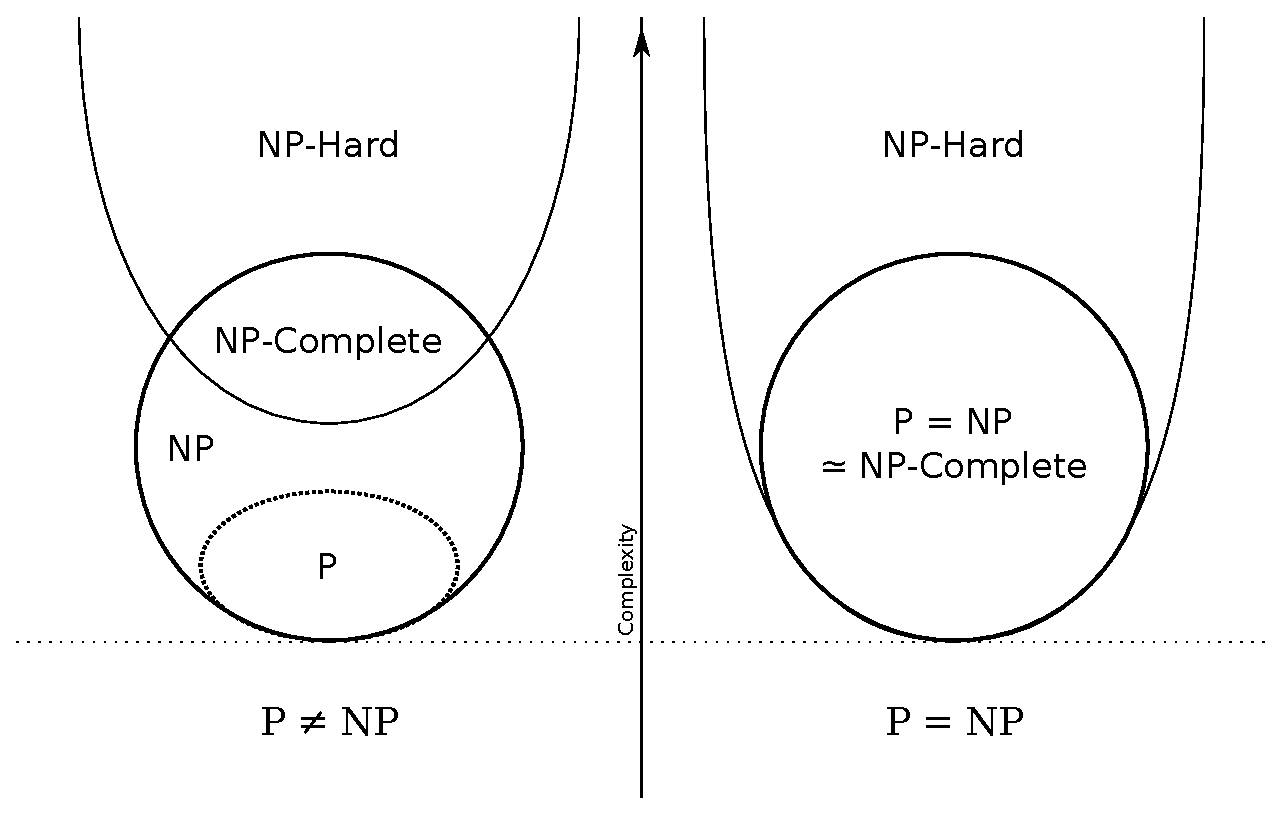
\includegraphics[scale=0.5]{P_np_np-complete_np-hard.eps}
\end{figure}

\subsection{判断一个问题是否是NP完全问题}
首先要记住几个经典的NP完全问题(重要的问题会在文末详细给出):布尔表达式可满足问题(SAT),合取范式的可满足问题(CNF-SAT),三元合取范式可满足问题(3-SAT),
k团问题(CLIQUE),k顶点覆盖问题(VERTEX-COVER),子集和问题(SUBSET-SUM),哈密顿回路问题(HAM-CYCLE),旅行商问题(TSP).

\textbf{Cook定理}说明SAT是NP完全问题,上述相邻的两个问题,前一个问题可通过多项式时间变换转化为后一个问题.

\textbf{证明一个问题$A$是否是NP完全问题}:假设已知问题$B$是NP完全问题,根据定义,只需证$A$是NP问题且
存在一个从$B$到$A$的多项式映射\footnote[1]{可以看出,要证明的问题$A$往往是非常难解的问题,比NP完全问题$B$还难.}. 

第一步:证明$A$是NP问题,即是否可以在多项式时间内给出\textbf{验证}是否为问题$A$的正确解.

第二步:找一个多项式时间内的映射,将问题$B$映射到问题$A$上即可.\\
\textbf{若只需证明$A$是NP难问题,则只需证明第二步.}

\ 

下面给出5个常用NP完全问题,可用于证明其它问题是NP完全问题:

\textbf{k团问题(CLIQUE)}:给定一个无向图$G=(V,E)$和一个正整数$k$,判定图$G$是否包含一个大小为$k$的团,
即是否存在,$V’\subset V,\ |V’|=k$且$\forall u, w\in V’$有$(u,w)\in E$.

\textbf{k顶点覆盖问题(VERTEX-COVER)}:给定一个无向图$G=(V,E)$和一个正整数$k$,判定是否存在$V’\subset V, |V’|=k$,
使得$\forall (u,v)\in E$有$u\in V’$或$v\in V’$. 若存在这样的$V’$,则称$V’$为图$G$的一个大小为$k$顶点覆盖.

\textbf{子集和问题(SUBSET-SUM)}:给定整数集合$S$和一个整数$t$,判定是否存在$S$的一个子集$S’\subset S$,使得$S’$中整数的和为$t$.

\textbf{哈密顿回路问题(HAM-CYCLE)}:给定无向图$G=(V,E)$,判定其是否含有哈密顿回路,即判定$G$是否存在经过$V$中各顶点恰好一次的回路.

\textbf{旅行商问题(TSP)}:给定一个无向完全图$G=(V,E)$及定义在$V\times V$上的一个费用函数$c$和一个整数$k$,
判定$G$是否存在经过$V$中各顶点恰好一次的回路,使得该回路的费用不超过$k$.
\end{document}